

\ifdefined\maindoc
% Do nothing (we are inside main.tex)
\else
\documentclass[12pt]{report}
\usepackage[a4paper,margin=1in]{geometry}
\usepackage[utf8]{inputenc}
\usepackage[T1]{fontenc}
\usepackage{amsmath,amssymb,amsthm}
\usepackage{booktabs}
\usepackage{setspace}
\usepackage{graphicx}
\usepackage{enumitem}
\usepackage{placeins}
\usepackage{hyperref}
\usepackage{array}
\usepackage[backend=biber,style=ieee,citestyle=numeric-comp,sorting=none]{biblatex}
\addbibresource{references.bib}
\newtheorem{definition}{Definition}
\onehalfspacing
\graphicspath{{figures/}}
% Standalone-only fallbacks so Chapter~\ref{...} renders as a number outside the main
% thesis. Under \maindoc these are skipped and the real labels in main.tex resolve.
% Numbers follow the agreed thesis order with this chapter as Chapter 3.
\makeatletter
\newlabel{ch:input-module}{{4}{1}{}{Doc-Start}{}}
\newlabel{ch:diamond-module}{{5}{1}{}{Doc-Start}{}}
\newlabel{ch:probability-toolkit}{{6}{1}{}{Doc-Start}{}}
\newlabel{ch:capacity-toolkit}{{7}{1}{}{Doc-Start}{}}
\newlabel{ch:critical-path}{{8}{1}{}{Doc-Start}{}}
\makeatother
\begin{document}
\title{Complex Processes as Directed Acyclic Graphs}
\fi

\section{Introduction}
\label{sec:model-intro}

The systems this thesis serves are flow-oriented. Water is abstracted,
treated and distributed. Power is generated, transformed and delivered.
Materials move through processing stages towards demand points, and
project activities complete in an order their dependencies dictate. In
each case the behaviour of the whole is organised by a directed movement
of something, supply, product, work or information, through a network of
components that pass it on.

The framework rests on a single model of such systems, defined in this
chapter and consumed unchanged by every module that follows. The model
fixes what a system becomes when it enters the framework, what its
components and their relationships mean, what a value attached to a
component can stand for, and which assumptions the later analyses inherit.
It closes with the three questions the model makes precise, which the
three analysis toolkits of Chapters~\ref{ch:probability-toolkit},
\ref{ch:capacity-toolkit} and~\ref{ch:critical-path} answer.

\section{From Process to Graph}
\label{sec:model-mapping}

A system enters the model through two identifications. Components become
nodes, and dependencies become directed edges. A component is whatever
unit of the system can meaningfully carry a value of its own, a pump, a
treatment stage, a substation, a task, and a dependency is the fact that
one component feeds, supplies or precedes another. Direction is not an
abstraction imposed on the system but a property read off it, because in
a flow-oriented process the relation between two connected components is
already asymmetric. Water leaves the intake and arrives at the pump, and
the pump does not supply the intake.

The model further requires that the directed edges form no cycle, and this
is the one modelling decision that needs defending rather than reading
off. For a large class of the target systems acyclicity is simply true.
Treatment trains, supply chains, assembly processes and project schedules
move material or work strictly forward, and a dependency cycle in a
schedule would be a planning error rather than a modelling choice. For
other systems it is an orientation of a richer reality. A distribution
pipe can carry water in either direction in principle, yet a network
operating around its design flows has a dominant direction on every pipe,
and orienting each edge by that dominant flow yields a directed acyclic
snapshot of the operating regime. What the orientation gives up is the
analysis of regimes far from the snapshot, flow reversals under unusual
demand, recirculation loops, feedback control, and the model excludes
these deliberately rather than approximating them. Figure~%
\ref{fig:model-mapping} shows the mapping on a small treatment process,
whose deliberate duplication of the treatment stage already displays the
structural phenomenon that Section~\ref{sec:model-roles} names.

\begin{figure}[htbp]
  \centering
  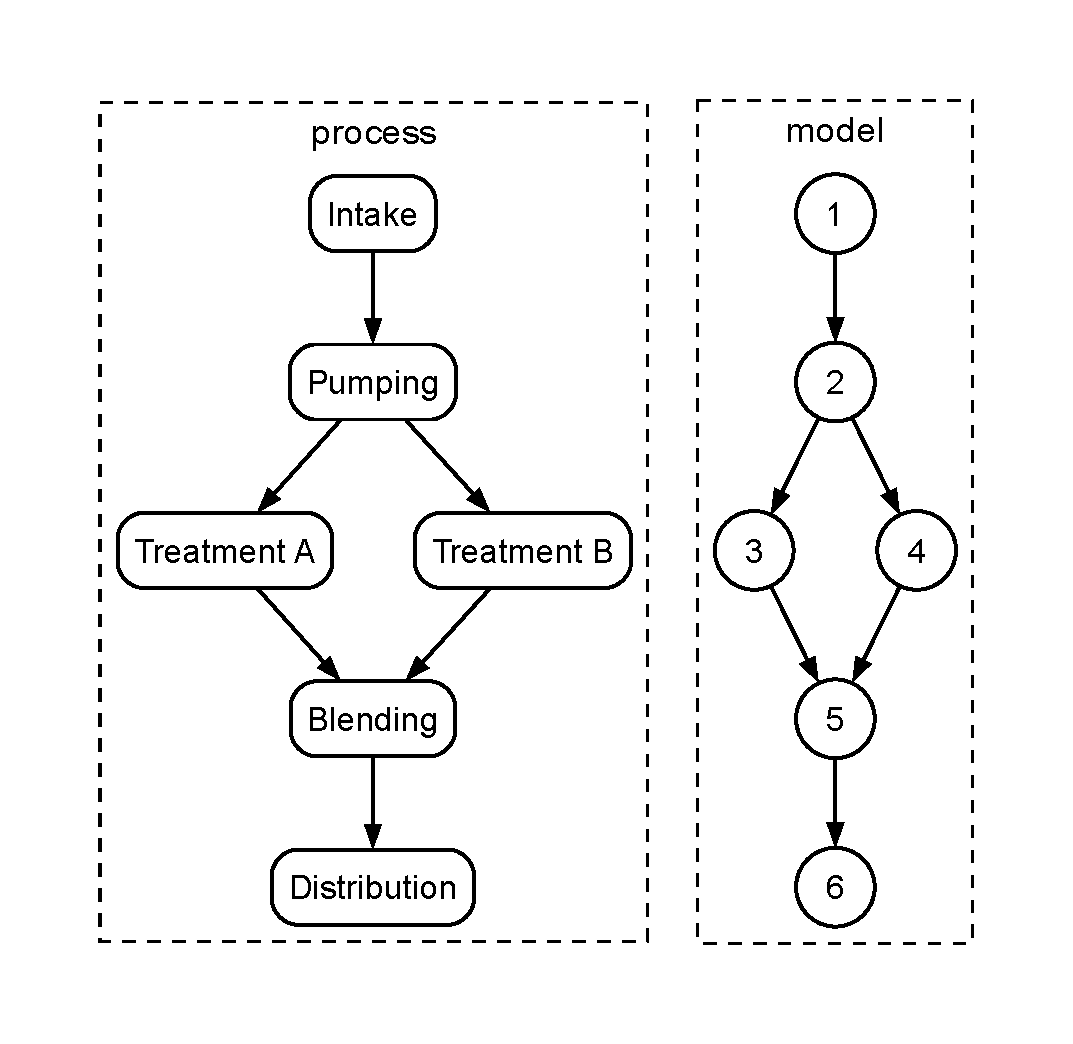
\includegraphics[width=0.78\linewidth]{fig01_mapping/fig01_mapping.pdf}
  \caption{A small treatment process and its model. Components become
  nodes, dependencies become directed edges, and the duplicated treatment
  stage becomes a pair of parallel routes that later reconverge.}
  \label{fig:model-mapping}
\end{figure}

\section{Node Roles}
\label{sec:model-roles}

Position in the network gives every node a role, and each role has a
physical reading. A node with no incoming edge is a source, the point
where supply, material or work enters the system, an intake, a generator,
the start of a project. A node with no outgoing edge is a sink, where the
system delivers, a demand point, an outlet, a completed handover. A node
that feeds two or more downstream components is a fork, and forks are how
systems distribute and, above all, how they build in redundancy, because
providing two routes to the same destination begins with one component
supplying two. A node fed by two or more components is a join, where
distributed flows gather, where assembled parts meet, and where redundant
routes come back together.

The last of those readings deserves emphasis, because it is a fact about
engineered systems rather than about graphs. Robust systems duplicate
deliberately, and duplicated routes must reconverge at the destination
they protect, so a well-designed network is dense with paths that separate
at a fork and meet again at a join while sharing the components upstream
of the fork. Whether that sharing matters depends on the question being
asked, and the chapters that ask the questions will return to it.
Chapter~\ref{ch:diamond-module} makes the pattern itself precise and
Chapter~\ref{ch:probability-toolkit} shows why, for one of the three
readings of the model, ignoring it produces wrong answers. Here it is
enough that reconvergence is a designed feature of the systems being
modelled, visible already in Figure~\ref{fig:model-roles}, not an
accident of drawing.

\begin{figure}[htbp]
  \centering
  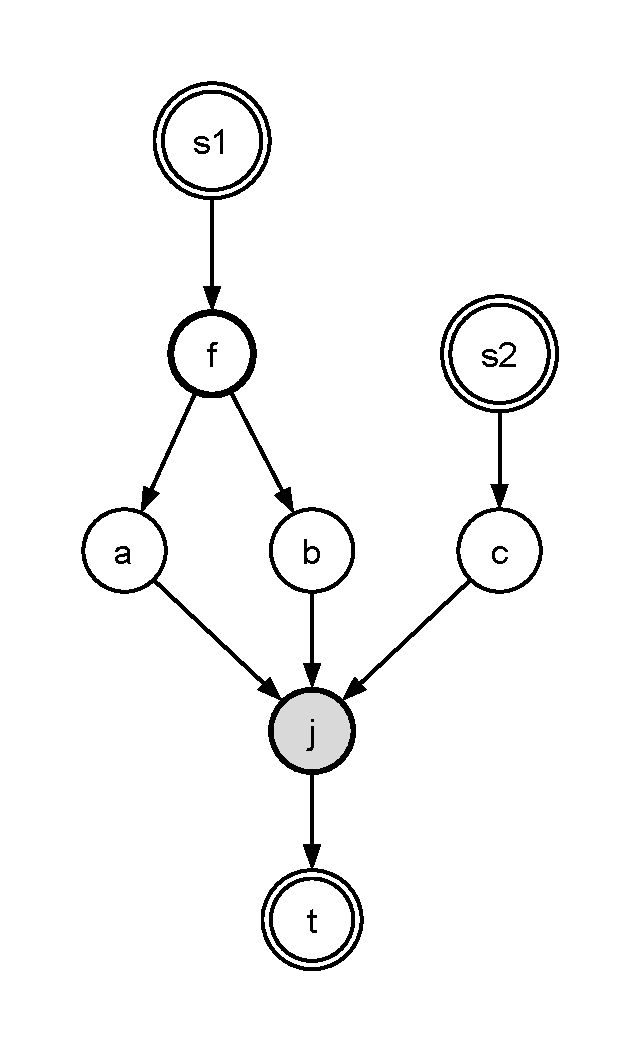
\includegraphics[width=0.5\linewidth]{fig02_roles/fig02_roles.pdf}
  \caption{Node roles on a small network. Double borders mark the source
  and the sink, the bold outline marks the fork, and the shaded node is
  the join where the redundant pair of routes reconverges alongside an
  independent supply.}
  \label{fig:model-roles}
\end{figure}

\section{The Formal Object}
\label{sec:model-formal}

\begin{definition}[Network model]
\label{def:model-network}
A system is modelled as a finite directed acyclic graph $G=(V,E)$ with
node set $V$ and edge set $E \subseteq V \times V$. The sources
$S \subseteq V$ are the nodes with no incoming edge and the sinks
$T \subseteq V$ the nodes with no outgoing edge. For a node $v$,
$\mathrm{Pa}(v)$ denotes its parents, the nodes with an edge into $v$,
and $\mathrm{Ch}(v)$ its children.
\end{definition}

\begin{definition}[Ancestry]
\label{def:model-ancestry}
A node $u$ is an ancestor of $v$ when a directed path leads from $u$ to
$v$, and a descendant when one leads from $v$ to $u$. The sets
$\mathrm{anc}(v)$ and $\mathrm{desc}(v)$ collect them, and throughout the
framework both are taken self-inclusively, so that
$v \in \mathrm{anc}(v)$ and $v \in \mathrm{desc}(v)$.
\end{definition}

\begin{definition}[Forks and joins]
\label{def:model-forks}
The forks of $G$ are $F = \{\, v : |\mathrm{Ch}(v)| \ge 2 \,\}$ and the
joins are $J = \{\, v : |\mathrm{Pa}(v)| \ge 2 \,\}$.
\end{definition}

These definitions are the shared vocabulary of the thesis. The chapters
that follow reference them rather than restate them, and
Table~\ref{tab:model-notation} collects the notation in one place.

\begin{table}[htbp]
\centering
\caption{Notation established by the network model.}
\label{tab:model-notation}
\small
\renewcommand{\arraystretch}{1.2}
\begin{tabular}{ll}
\toprule
Symbol & Meaning \\
\midrule
$G=(V,E)$ & the system as a finite DAG \\
$S$, $T$ & sources (no incoming edge), sinks (no outgoing edge) \\
$\mathrm{Pa}(v)$, $\mathrm{Ch}(v)$ & parents and children of $v$ \\
$\mathrm{anc}(v)$, $\mathrm{desc}(v)$ & ancestors and descendants, self-inclusive \\
$F$, $J$ & fork nodes (fan-out $\ge 2$), join nodes (fan-in $\ge 2$) \\
\bottomrule
\end{tabular}
\end{table}

\section{Information on the Network}
\label{sec:model-information}

The model separates what the network is from what is asked of it. The
topology of Definition~\ref{def:model-network} is fixed once per system,
and an analysis attaches values to its nodes and edges whose meaning
depends on the question. Under the probabilistic reading a node's value
is the probability that the component operates and an edge's value the
probability that the handover between its endpoints succeeds, so the
network describes what survives failure. Under the schedule and cost
reading the values are durations or costs, of the component's own
processing and of the transfer along each dependency, so the network
describes when things complete and what they accumulate. Under the
capacity reading the values are throughput limits, and the network
describes how much can be carried. Three readings of one topology are
three different analyses, and keeping the topology common across them is
what allows a single system model to answer questions that are usually
asked of three separate models \cite{ouyang2014interdependent}.

How well a value is known is a further axis, independent of what it
means. A deterministic value asserts full knowledge, and is the right
form for design constants and well-measured components. An interval
asserts only bounds, and is the honest form when data is sparse, when a
manufacturer quotes a tolerance, or when experts will commit to a range
but not a number. A probability box bounds a distribution rather than a
value, and carries partial statistical knowledge, measurements enough to
constrain a curve without fixing it. The framework propagates all three
forms through the same analyses, so the choice among them reflects the
state of knowledge about the system rather than the limits of the tool.

\section{Assumptions and Limits}
\label{sec:model-assumptions}

The model buys its tractability with four assumptions, and each is a
limit on what the answers mean. Component behaviours are independent, so
a common cause that fails several components together is not represented
and must be modelled explicitly as a shared upstream node where it
matters. Under the probabilistic reading a component is binary,
operational or failed, and degraded intermediate states are outside the
model. The topology is static over the analysis horizon, so
reconfiguration during operation is a sequence of separate analyses
rather than one. And the acyclicity of Section~\ref{sec:model-mapping}
prices out feedback and reversal, which is a property of the operating
snapshot being analysed rather than of the physical assets. None of
these assumptions is hidden in an algorithm, and every result in the
later chapters is conditional on exactly this list.

\section{Three Questions}
\label{sec:model-questions}

The model makes three questions precise, and the thesis answers them in
turn. Under the probabilistic reading the question is whether information
survives the network, with what probability a node is reached from the
sources despite component failures, and it is answered by the Probability
Propagation Toolkit of Chapter~\ref{ch:probability-toolkit}. Under the
capacity reading the question is how much the network can deliver, where
the limits bind and what relieving them buys, answered by the Capacity
Flow Toolkit of Chapter~\ref{ch:capacity-toolkit}. Under the schedule and
cost reading the question is when and at what accumulation the network
completes, which dependencies set that outcome and which have room to
move, answered by the Critical Path Toolkit of
Chapter~\ref{ch:critical-path}.

Before any of the three can be asked, the model itself must be built from
the heterogeneous descriptions in which real systems arrive, which is the
work of Chapter~\ref{ch:input-module}, and for the probabilistic question
the reconvergent structure of Section~\ref{sec:model-roles} must be
identified and organised, which is the work of
Chapter~\ref{ch:diamond-module}. The two are preprocessing in the strict
sense, performed once per system, and everything after them is a reading
of the object this chapter has defined.

\ifdefined\maindoc
% do nothing
\else
\printbibliography
\end{document}
\fi
